%start preamble
\documentclass[paper=a4,fontsize=11pt]{scrartcl}%kind of doc, font size, paper size

\usepackage{fontspec}
\defaultfontfeatures{Ligatures=TeX}
%\setsansfont{Liberation Sans}
\usepackage{polyglossia}	
\setdefaultlanguage[spelling=new, babelshorthands=true]{german}
		
\usepackage{amsmath}%get math done
\usepackage{amsthm}%get theorems and proofs done
\usepackage{graphicx}%get pictures & graphics done
\graphicspath{{pictures/}}%folder to stash all kind of pictures etc
\usepackage{amssymb}%symbolics for math
\usepackage{amsfonts}%extra fonts
\usepackage []{natbib}%citation style
\usepackage{caption}%captions under everything
\usepackage{listings}
\usepackage[titletoc]{appendix}
\numberwithin{equation}{section} 
\usepackage[printonlyused,withpage]{acronym}%how to handle acronyms
\usepackage{float}%for garphics and how to let them floating around in the doc
\usepackage{cclicenses}%license!
\usepackage{xcolor}%nicer colors, here used for links
\usepackage{wrapfig}%making graphics floated by text and not done by minipage
\usepackage{dsfont}
\usepackage{stmaryrd}
\usepackage{geometry}
\usepackage{hyperref}
\usepackage{fancyhdr}
\usepackage{menukeys}

%settings colors for links
\hypersetup{
    colorlinks,
    linkcolor={blue!50!black},
    citecolor={blue},
    urlcolor={blue!80!black}
}

\definecolor{pblue}{rgb}{0.13,0.13,1}
\definecolor{pgreen}{rgb}{0,0.5,0}
\definecolor{pred}{rgb}{0.9,0,0}
\definecolor{pgrey}{rgb}{0.46,0.45,0.48}

\pagestyle{fancy}
\lhead{Netzwerke Übung (WiSe 2019/20)}
\rhead{FB 4 -- Angewandte Informatik\\ HTW-Berlin}
\lfoot{Übungsblatt 05 -- Geroutete Netzwerke}
\cfoot{}
\fancyfoot[R]{\thepage}
\renewcommand{\headrulewidth}{0.4pt}
\renewcommand{\footrulewidth}{0.4pt}

\lstdefinestyle{Bash}{
  language=bash,
  showstringspaces=false,
  basicstyle=\small\sffamily,
  numbers=left,
  numberstyle=\tiny,
  numbersep=5pt,
  frame=trlb,
  columns=fullflexible,
  backgroundcolor=\color{gray!20},
  linewidth=0.9\linewidth,
  %xleftmargin=0.5\linewidth
}

\newlength\labelwd
\settowidth\labelwd{\bfseries viii.)}
\usepackage{tasks}
\settasks{counter-format =tsk[a].), label-format=\bfseries, label-offset=3em, label-align=right, label-width
=\labelwd, before-skip =\smallskipamount, after-item-skip=0pt}
\usepackage[inline]{enumitem}
\setlist[enumerate]{% (
labelindent = 0pt, leftmargin=*, itemsep=12pt, label={\textbf{\arabic*.)}}}


%%here begins the actual document%%
\newcommand{\horrule}[1]{\rule{\linewidth}{#1}} % Create horizontal rule command with 1 argument of height

\DeclareMathOperator{\id}{id}

\begin{document}
\begin{center}
\Large{\textbf{Hausaufgaben 05 -- Geroutete Netzwerke}}\\
\end{center}
Nachdem Sie in der letzten Übung einige Grundlagen im Bereich Linux und Netzwerktechnik kennengelernt haben, soll im Folgenden darauf aufbauend Ihr Wissen erweitert werden. Mit diesem Hausaufgabenblatt sollen die Fundamente für die Umsetzung eines einfachen, statisch gerouteten Netzwerks gelegt werden.

\begin{center}
\Large{\textbf{Aufgabe A -- Routing}}
\end{center}
\vskip0.25in
Nachdem Sie im letzten Übungsblatt Ihr Netzwerk durch einen Switch verbunden haben und hierdurch Ihre Kommunikation aufbauten, "'wandern" Sie im kommenden Übungsblatt im OSI-Modell eine Schicht weiter nach oben. Es soll folglich ein Netzwerk geplant und umgesetzt werden, das auf Routing setzt -- der Router ist fortan zentrale Anlaufstelle für die Kommunikation!\\
Diese Umsetzung hat den Vorteil, dass der Router Pakete über Netzgrenzen hinweg vermitteln kann. Ihr kleines, abgeschottetes Netzwerk kann über die bisherigen Grenzen hinweg kommunizieren.
\begin{enumerate}
	\item Im Übungsblatt 03 haben Sie sich bereits mit Routing beschäftigt. Rekapitulieren Sie Ihr Wissen!
	\item Lesen Sie Kapitel 4.3 in \cite[S. 320ff]{Kurose2012} zum Thema Routing und Router.
	\item Was sind die Aufgaben eines Routers. Wie erfolgt, im Groben, die Umsetzung des Routings?
	\item Machen Sie sich klar, wie Router und \emph{IP}-Protokoll zusammenhängen.
	\item In welcher Schicht des OSI-Modells würden Sie einen Router einordnen? (Begründung!)
	\item Wie haben sich bis jetzt Ihre VMs gefunden? Woher "'wussten" diese, an welches Gerät die Ethernet-Frames zu schicken waren? Wie spielt hier Ihre eigene IP-Adresse und Subnetzmaske mit hinein? Bzw. spielt diese auf Hardwareebene eine Rolle?
	\item Woher weiß ein \textit{Host} (Endknoten), wann er ein Paket direkt adressieren kann und wann er es an Router/Gateway weiter schicken muss?
	\item Woher weiß ein \textit{Router} (Zwischenknoten), wann er ein Paket weiter schicken soll und wann nicht?
\end{enumerate}

\begin{center}
\Large{\textbf{Aufgabe B -- Planung des Routing zwischen Netzen}}
\end{center}
\vskip0.25in
Im vorigen Aufgabenblatt haben Sie zu den IP-Adressen auch eine Netzwerkmaske konfiguriert. Diese Netzwerkmaske legt fest, welche Rechner im gleichen (Sub-)Netz liegen und somit direkt angesprochen werden können. Daraus folgt aber auch, dass bestimmte Rechner außerhalb Ihres Netzes nicht direkt angesprochen werden können. Diese können via Router/Gateway erreicht werden.\\
Wir wollen in einem ersten Schritt selber einen Router betreiben, um über unsere kleinen Netze hinweg zu kommunizieren. Dazu erweitern Sie Ihr Wissen aus dem vorigen Übungsblatt, sodass Ihr Netzwerk im Labor "'wachsen" kann.
\begin{enumerate}
	\item Früher wurden Klassen von Adressen genutzt, heute das \emph{CIDR (Classles Inter Domain Routing)}. Worin unterscheiden sich \emph{CIDR} und klassenbasierte Adressen?
	\item Recherchieren Sie, warum sich dies änderte! (Kapitel 4.4.2 \cite[S. 338ff]{Kurose2012} oder RFC 4632)
	\item Recherchieren Sie wie die Syntax der klassenbasierten Notation aussieht und geben Sie einige Beispiele für die Notation.
	\item Recherchieren Sie wie die Syntax der \emph{CIDR}-Notation aussieht und geben Sie einige Beispiele für die Notation.
	\item Wie in der letzten Übung arbeiten Sie in Gruppen von je vier Studierenden.\\
	Um zwischen den beiden lokalen Netzwerken kommunizieren zu können, benötigen Sie einen Router. Einer der VMs soll diese Aufgabe übernehmen.\\
	Die Rechner müssen so konfiguriert werden, dass sie wissen wohin die Pakete geschickt werden -- das heißt: Pakete die nicht in das eigene lokale Netzwerk gehören, werden über den Router in die externen Netzwerke weitergereicht. Die Umsetzung entspricht schematisch der Abb. \ref{sketch_lan}.
	\begin{figure}[H]
	\centering
	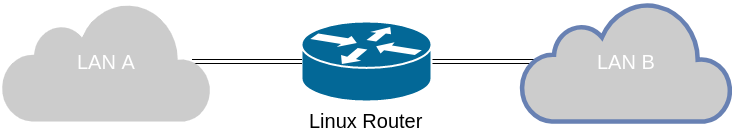
\includegraphics[scale=0.35]{lan}
	\caption{Skizze des Netzwerkes bestehend aus zwei LANs und einem Linux-Router}
	\label{sketch_lan}
	\end{figure}
	\begin{tasks}
		\task Unterteilen Sie Ihre Gruppe, sodass sich im Idealfall zwei VMs in einen lokalen Netzwerk $A$ und zwei VMs im lokalen Netzwerk $B$ befinden.
		\task Skizzieren Sie Ihre lokalen Netzwerke, sowie das gesamte Netzwerk (Nutzen Sie geeignete Symbole -- s. letztes Übungsblatt).
		\task Vergeben Sie entsprechende \emph{IPv4}-Adressen und kleinst mögliche Subnetzmasken auf der Skizze. Wählen Sie ein ähnliches Adressschema, wie in der letzten Laborübung.
		\task Planen Sie ebenso den Router mit entsprechenden \emph{IPv4}-Adressen auf der Skizze ein.\\
		Achten Sie darauf, dass der Router als Verbindungsstück (Intermediate-Node/ Zwischenknoten) zwischen Ihren beiden Netzen fungiert und dementsprechend beide Netzwerke kennen muss. Das heißt, der Router muss \textbf{zwei} \emph{IPv4}-Adressen haben, jeweils eine pro Netzwerk.
	\end{tasks}
\end{enumerate}

\begin{center}\Large{\textbf{Aufgabe C -- Planung des Backbones}}\end{center}\vskip0.25in
Aufbauend auf den kleinen LANs pro Tischreihe, soll eine größere Netzwerkinfrastruktur aufgebaut werden -- ein sogenanntes Backbone. Die kleinen separaten Netzwerke werden verknüpft. Darüber hinaus sollen Sie für einen Anschluss an das Internet sorgen (der sogenannte \emph{Uplink}).\\
\footnote{Backbone-Routing wird auch an den großen Internet-Knoten umgesetzt (diese werden als Internet-Exchange-Point -- IXP bezeichnet), wie etwas dem \emph{DECIX} (\url{https://www.de-cix.net/}).}
Im wesentlichen erweitern Sie den Aufbau Ihres Netzwerkes -- jedes LAN bekommt lediglich einen extra (Backbone-) Router. Das Netzwerk soll im wesentlichen dem Ausschnitt in Abb. \ref{backbone} entsprechen.
	\begin{figure}[H]
	\centering
	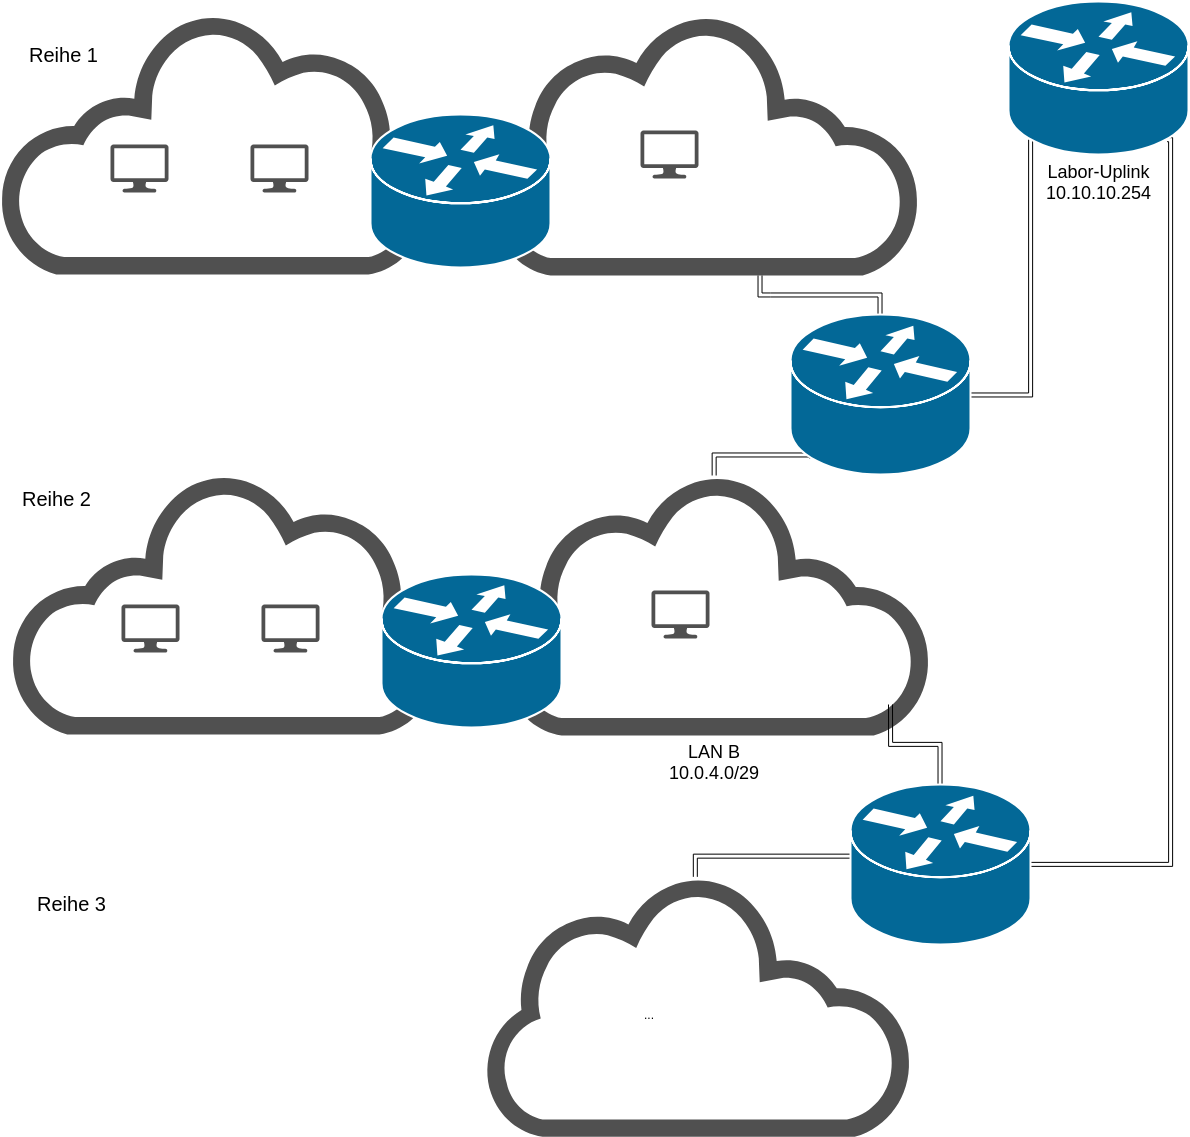
\includegraphics[scale=0.25]{backbone}
	\caption{Skizze (auszugsweise) des Netzwerks bestehend aus fünf Bankreihen á zwei LANs, sowie den Backbone-Routern und dem Uplink.}
	\label{backbone}
	\end{figure}
Folgendes Adressschema gilt:
\begin{table}[H]
\caption{Adressschema für das Labor}
\label{adress_scheme}
\centering
\begin{tabular}{|c|c|}\hline
 & \textbf{IP  || IP-Range} \\ \hline
 $LAN_X$ & 10.0.$X$.Y/Size \\ \hline
 Backbone & 10.10.10.100 + $\rho$ (Rho)\\ \hline
 Labornetz & 10.0.0.0/8 \\ \hline
 Uplink & 10.10.10.254 \\ \hline
 DNS & 10.10.10.254 \\ \hline
\end{tabular}
\end{table} 
$LAN_X$ bezeichnet die beiden Netzwerke (Ihre Bankreihe mit je zwei Subnetzen), wobei der Wert $X$ der Reihe nach hochgezählt wird. D.h. Bankreihe eins: $LAN_{1}$, Bankreihe zwei: $LAN_{2}$ etc.\\ Beachten Sie, dass Sie innerhalb eines LANs/Subnetzes festlegen müssen wo ein Netzsegment beginnt und endet! 
	\begin{tasks}
		\task Planen Sie entsprechend der Skizze Ihr Netzwerk. D.h. planen Sie entsprechende
		\emph{IPv4}-Adressen, Subnetzmasken und Router ein.
		\task Skizzieren Sie Ihre lokalen Netzwerke, sowie das gesamte Netzwerk mitsamt der Router (Nutzen Sie geeignete Symbole).
		\task Planen Sie ebenso den Backbone-Router ein.
		\task Ebenso sollten Sie den Uplink einplanen! Um diesen umsetzen zu können, müssen Sie 		
		auf dem Backbone eine \emph{IPv4}-Adresse innerhalb des Labors definieren. Die Adresse sollte daher folgendes Schema besitzen: $10.10.10. 100 + \rho$, wobei $\rho$ Ihrer Bankreihe entspricht.
		\task Wie muss die Subnetzmaske für die $10.10.10. 100 + \rho$ Adresse aussehen?\\
		Anm.: Sie müssen bedenken, dass das Backbone mit dieser Adresse im gleichen LAN wie der Uplink sein muss.
	\end{tasks}

\begin{center}
\Large{\textbf{Aufgabe D -- Tools \& OS}}
\end{center}
\vskip0.25in

\begin{enumerate}
	\item Seit der letzten Übung kennen Sie schon einige grundlegende Befehle, um das Netzwerkinterface eines unixoiden Betriebssystems zu konfigurieren. Dieses Wissen soll nun erweitert werden.\\
	Hierfür schauen wir in die bekannten Werkzeugkästen \emph{iproute2} und \emph{net-tools}.
	\begin{tasks}(1)
		\task Recherchieren Sie, welches Werkzeug aus \emph{iproute2} genutzt werden kann um Routen zu setzen.\\
		Notieren Sie sich die Syntax und was die Parameter bewerkstelligen.
		\task Analog dazu: Wie werden Routen mithilfe der \emph{net-tools} konfiguriert?
		\task Recherchieren Sie beispielhaft wie eine persistente Lösung aussähe. Kommentieren Sie 
		Ihr Beispiel anschließend, sodass Sie wissen was die einzelnen Wörter/Token bedeuten.
	\end{tasks}
	\item Gateways \& Router -- Gateways sind im allgemeinen nicht das Gleiche wie Router. Auch unter den Gateways gibt es Unterscheidungen.
	\begin{tasks}(1)
		\task Recherchieren Sie worin sich Router und Gateways unterscheiden.
		\task Beim aufsetzen des Netzwerkes kann unterschieden werden zwischen \emph{Gateways} und \emph{Default-Gateways}. Recherchieren Sie diese Unterscheidung.
	\end{tasks}
	\item Im vorigen Übungsblatt arbeitete Ihr Netzwerk mithilfe eines Switches. Alle Knoten des Netzwerkes waren innerhalb eines Segments (LAN). Daher konnte Sie nur innerhalb Ihres Netzwerkes kommunizieren, darüber hinaus aber nicht. Mithilfe eines Routers erweitern Sie die Reichweite Ihres Netzwerkes.\\ 
	Routing ist wesentlich komplexer als das direkte adressieren von Frames/Paketen, da in der Regel Wege zwischen Endknoten durch ein Netzwerk gefunden werden müssen (Route). Aufgrund dieser Tatsache müssen Sie ein wenig tiefer in das Betriebssystem schauen.
	\begin{tasks}(1)
	\task Lesen Sie Kapitel 4.1.1. \cite[S. 308ff]{Kurose2012} zum Thema Routing und Forwarding. Worin unterscheiden sich diese Mechanismen?
	\task Lesen Sie folgenden Artikel: \url{https://www.techrepublic.com/article/understand-the-basics-of-linux-routing/} -- Besonders ab dem Abschnitt "'Understanding Routing".
	\task Der Betriebssystemkern (Kernel) stellt die Infrastruktur für das Routing bereit. Nennen Sie die hierfür maßgebliche Kernel-Structure. (Steht im ersten Satz des Understanding Routing Absatzes!) Was ist die Aufgabe dieser Datenstruktur?
	\task Welchen Kernel-Parameter müssen Sie aktivieren (bzw. welche Datei im \path{/proc/sys} Verzeichnis müssen sie editieren), sodass das IP-Forwarding aktiviert wird? Welche Möglichkeiten zum Editieren dieser Datei haben Sie?
	\task In welcher Konfigurationsdatei müssen Sie einen Eintrag vornehmen, so das das Routing dauerhaft beim Systemstart aktiviert bleibt? Notieren Sie sich beispielhaft (auszugsweise) wie dies aussehen kann.
	\end{tasks}
	\item Das Internet Control Message Protocol (\emph{ICMP}) wurde in Übung 04 bereits besprochen. Rekapitulieren Sie Ihr Wissen!
	\item Recherchieren Sie welchen Hinweis Ihnen dabei die Folgenden \emph{ICMP}-Messages geben. Wo wird jeweils der Fehler in der Konfiguration liegen?
	\begin{tasks}(1)
		\task Connect: network is unreachable
		\task Destination Host Unreachable
		\task Destination Network Unreachable
		\task keine Antwort auf ein Ping
	\end{tasks}
	\item Zwei weitere bekannte Netzwerkanalyse-Tools sind \emph{netstat} (aus \emph{net-tools}) und \emph{ss} (aus der \emph{iproute2}-Werkzeugsammlung).
	\begin{tasks}
		\task Recherchieren Sie die wesentliche Funktionen von \emph{netstat}, sowie \emph{ss}.
		\task Notieren Sie sich anhand von Beispielen die Syntax der eben genannten Tools. 
	\end{tasks}
	\item \emph{iptables} wird unter Linux allgemein als Firewall-Tool genutzt.\\
	In der kommenden Übung übernimmt \emph{iptables} eine etwas andere Aufgabe. Es sorgt zunächst dafür, dass unsere VMs via \emph{NAT}\footnote{Um genau zu sein: SNAT} Pakte in das Internet leiten können. Wir erweitern das Backbone also zu einem \emph{NAT}-Gateway -- dies übersetzt unsere privaten IP-Adressen auf Adressen des Labors. Mit dem selben Verfahren wird die Laboradresse auf dem Uplink auf eine IP-Adresse des Hochschulnetzes abgebildet. 
	\begin{tasks}
		\task Recherchieren Sie entweder unter \cite[S. 349f]{Kurose2012} oder mithilfe folgenden Links was \emph{NAT} ist und warum dies unter \emph{IPv4} genutzt wird.\\
		\url{https://en.wikipedia.org/wiki/Network_address_translation}
		\task Machen Sie sich im groben klar, wie \emph{NAT} umgesetzt wird.
		\task Recherchieren Sie kurz welche \emph{NAT}-Varianten es gibt. 
		\task \textbf{Fakultativ:} Mit sehr hoher Wahrscheinlichkeit nutzt auch Ihr Router/Modem \emph{NAT}, wie wird dies hier umgesetzt?
		\task Recherchieren Sie was unter einer Firewall im wesentlichen verstanden wird.
		\task Machen Sie sich klar, wie eine Firewall im Groben umgesetzt wird -- wie setzt eine Firewall seine Regeln um.
		\task \emph{iptables} kann genutzt werden, um die privaten Adressen auf öffentliche zu übersetzen. Lesen Sie folgenden Artikel:\\
		\url{https://access.redhat.com/documentation/en-US/Red_Hat_Enterprise_Linux/4/html/Security_Guide/s1-firewall-ipt-fwd.html}\\
		Versuchen Sie den Inhalt wirklich komplett zu verstehen. Notieren Sie sich alle notwendigen Schritte um das Masquerading via \emph{iptables} einzuschalten.
		\task \emph{iptables} unterstützt sowohl \emph{SNAT} (One-to-Many-NAT) als auch \emph{DNAT}. Recherchieren Sie kurz worin sich beide Arten unterscheiden.
	\end{tasks}
\end{enumerate}

\begin{center}\Large{\textbf{Aufgabe E -- IPv6}}\end{center}\vskip0.25in
Im letzten Übungsblatt haben Sie bereits eine kurzen Blick auf \emph{IPv6} geworfen. Momentan wird immer noch vornehmlich auf das "'alte" Internetprotokoll gesetzt, Sie jedoch sollen auch fit für die Zukunft sein.
\begin{enumerate}
	\item Rufen Sie sich erneut ins Gedächtnis welche Vorteile \emph{IPv6} mit sich bringt.
	\item Recherchieren Sie zunächst den Adressaufbau von \emph{IPv6}. Aus welchen Teilen bestehen \emph{IPv6}-Adressen und welche Aufgabe/Zweck erfüllen die einzelnen Bestandteile.
	\item Machen Sie sich anschließend mit der Adressnotation vertraut! Notieren und kommentieren Sie einige Beispiele.
	\item Wie \emph{IPv4} hat auch \emph{IPv6} private Adressbereiche. Welche sind dies und wie ist deren Aufbau?
	\item Recherchieren Sie wie die \emph{CIDR}-Notation für \emph{IPv6} aussieht.
	\item Im Gegensatz zu \emph{IPv4} muss \emph{IPv6} zwangsläufig mehrere Addressen auf einem Interface definieren. Die erste verfügbare Adresse ist eine \texttt{link locale}-Adresse. Machen Sie sich klar, wie diese zu finden ist. Diese Adresse folgt immer dem Schema  \texttt{fe80::/10}.\\
	Machen Sie sich ebenso klar, warum diese Adresse von Nöten ist.
	\item Recherchieren Sie wie die Vergabe von \emph{IPv6}-Adressen und das setzen von \emph{IPv6}-Routen aussieht. Machen Sie sich auch hier klar, was die einzelnen Bestandteile der Kommandos bewirken!
	\item Um das Routing zu ermöglichen benötigen Sie genau wie bei \emph{IPv4} eine Routing-Tabelle. Recherchieren Sie entsprechend, wie das Forwarding (für das Routing) zu aktivieren ist.
\end{enumerate}
\bibliographystyle{plain}
\bibliography{sources}
\end{document}